%! TEX root = ../main.tex
\documentclass[../main.tex]{subfiles}
\begin{document}
\section{Anwendungen in Forschung und Industrie}
\label{sec:anwendungen}
\begin{figure}[H]
	\centering
	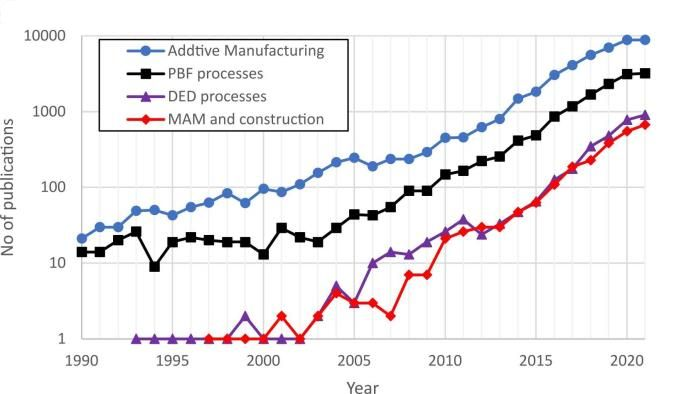
\includegraphics[width=1\textwidth]{search5}
	\ccaption{Anzahl an wissenschaftlichen Artikeln und Publikationen zum Thema 3D-Druck}{adaptierte Grafik, von \protect\cite{KANYILMAZ2022102541} entnommen}
	\label{img:search_5}
\end{figure}
Wie aus Abb. \ref{img:search_5} erkennbar ist, ist die Nachfrage und Forschung für die Anwendung des 3D-Drucks, besonders für die \acrlong{slm}- und \acrfull{pbf}-Prozesse, stark angestiegen in den letzten beiden Jahrzehnten.

\begin{figure}[H]
	\centering
	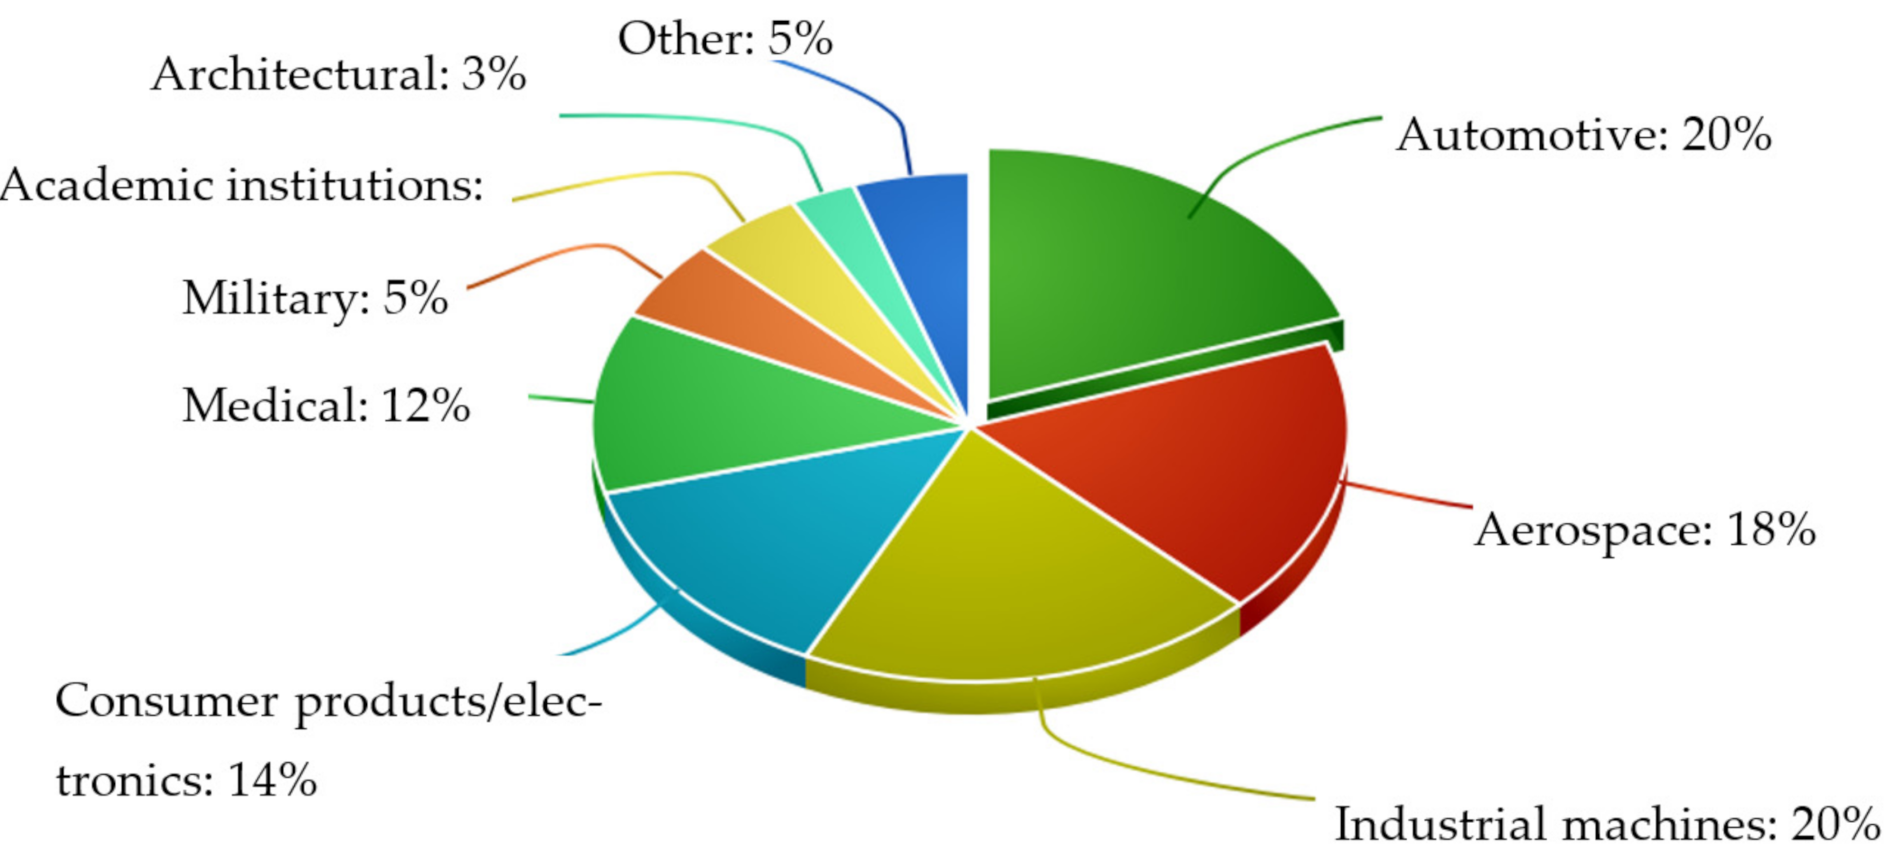
\includegraphics[width=1\textwidth]{am_shares}
	\ccaption{Anteile verschiedener Anwendungsgebiete im \acrshort{am} (Stand 2017) }{Grafik von \protect\cite{app11031213} entnommen}
	\label{img:am_shares}
\end{figure} 
\subsection{Forschung}
Der Metall-3D-Druck erfreut sich in Forschungs- und Entwicklungs-Anwendungen sehr großer Beliebtheit, da durch solche Technologien eine schnelle \say{Iterationszeit}, also Zeit zwischen der Produktion von Designs und Ideen, ermöglicht wird. Zudem kann viel Material im Vergleich zu subtraktiver Produktion eingespart werden. Es ist nicht mehr nötig an die Umsetzbarkeit durch Fräßen, Bohren und Drehen zu denken, da mit einem Metall-3D-Drucker viel weniger Limitierungen existieren (es können vollständig verdeckte Kühlkanäle durch einen Teil gelegt werden, welche mit konventionellen Methoden unmöglich wären).
\subsubsection*{Medizinische Implantate}
\label{sec:medizin}
In der Medizin wird 3D-Druck hauptsächlich im Kontext der Erschaffung von Knochen-Implantaten erforscht. Mithilfe eines Computer-Tomographie-Scans wird ein Abbild des Knochens digital erschaffen, welches von einem \acrshort{am}-Ingenieur nach-bearbeitet und aufbereitet wird wie in \ref{img:medical} erkennbar ist. Viele Aspekte dieser Aufbereitung werden mit Computer-gestützten Algorithmen durchgeführt, um sie an die Form des Knochens anzupassen.\parencite{doi:10.1146/annurev-bioeng-082020-032402}

\begin{figure}[H]
	\centering
	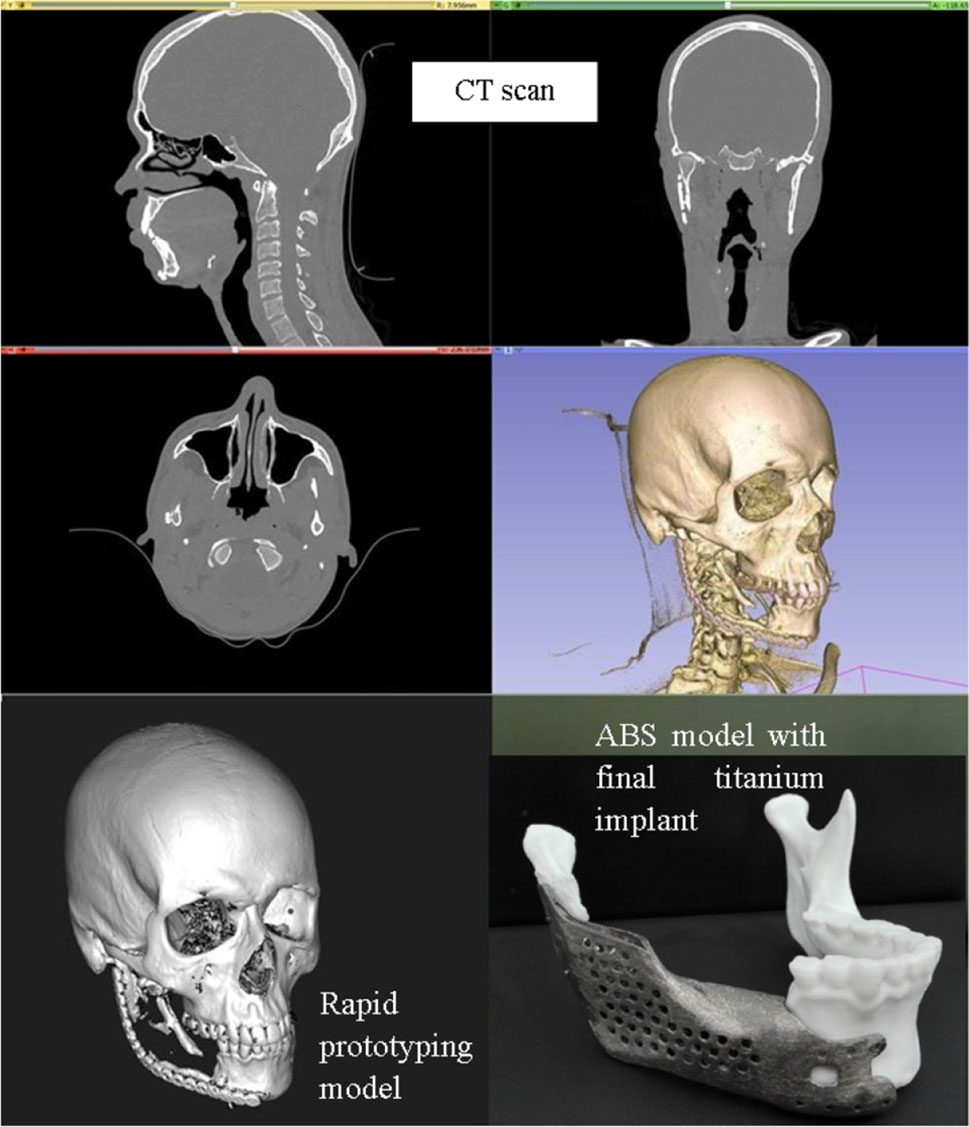
\includegraphics[width=.5\textwidth]{medical_2}
	\ccaption{Ablauf der Aufbereitung eines CT-gescannten Kiefer-Implantats}{Grafik von \protect\cite{LEE20221648} entnommen}
	\label{img:medical}
\end{figure} 
Zudem sind die Implantate zu meist mit verschiedenen \it{Lattice}-Strukturen ausgefüllt und anderen Methoden der Gewicht-Verringerung optimiert worden, um Material zu sparen und dem Körper mehr Oberfläche zu geben, um sich damit zu verbinden. Hauptsächlich werden als Material Titan-Legierungen verwendet, wie z.B. Ti-6Al-4V, da diese gut verträglich für den Körper sind, korrosions-resistent sind und leichter sind als die meisten Stähle.
($\rho_{Titan} = \qty{4.2}{\gram\per\centi\meter\cubed}, \rho_{Stahl} = \qty{8.05}{\gram\per\cm\cubed}$). \parencite{steel12709, titanium6al4v}
Da diese Implantate sehr präzise Spezifikationen einzuhalten haben, wird hier ausschließlich der \acrlong{slm} Prozess verwendet, da \acrshort{lmd} zu inkonsistent ist in diesem Maßstab. Dennoch ist eine Nachbearbeitung und Anpassung vor und während der Operation fast immer nötig um den perfekten Sitz des Knochenersatzes zu garantieren.\parencite{doi:10.1146/annurev-bioeng-082020-032402}

Für Last-tragende Knochen müssen die Implantate wärme-behandelt werden, um die gewünschte Stabilität und Flexibilität zu erreichen, welche ein Brechen des Implantates nach der Einsetzung verhindern soll.

Weiters ist eine Beschichtung der Teile oft von Vorteil, um die Entzündungswahrscheinlichkeit und Gefahr der Ablehnung des Implantats durch den Körper zu minimieren. Oft werden hierzu Materialien wie \ce{Ca10(PO4)6(OH)2 (Hydroxylapatit)} verwendet, welche in Verfahren wie \acrfull{pacvd} oder \it{RF-Magnetron-Sputtering} aufgetragen werden in dünnen Schichten (einige nm - $\mu$m).\parencite{Chudinova2016}

 
\subsection{Industrie}
\subsubsection{Reparatur und OOP-Ersatzteil-Produktion}
Das durchschnittliche Alter industriell verwendeter Maschinen liegt bei 15+ Jahren \parencite{lifespan_1}, wobei die meisten dieser Maschinen sowie auch ihre Ersatzteile bereits \acrfull{oop} sind. 
Restbestände sind nur mehr für sehr hohe Preise verfügbar und mit logistischem Aufwand verbunden. 
Oft ist es dadurch effizienter für Firmen neue Maschinen anzuschaffen, obwohl die existierenden Geräte bis auf einzelne Bauteile noch gut funktionieren. 
Auch logistische Probleme sind ein großer hindernder Faktor für den Zugriff auf Ersatzteile, besonders in Bereichen wie Schiffsfahrt oder Luftfahrt. Der Transport eines Schiffspropellers, welche zumeist mehrere Tonnen wiegen, ist logistisch sehr kompliziert und teuer.  
Mithilfe eines LMD-ähnlichen Prozesses ist es aber möglich besagten Teil lokal zu produzieren \parencite{ship_1} und dabei Transport- und Lagerkosten sowie auch viel Zeit zu sparen. 

Bei dem obigen Beispiel wird der Teil komplett neu produziert. 
Eine für viele Industrien realistischere Option ist die Reparatur eines beschädigten Teils. Für eine komplette Reproduktion wäre ein \acrshort{cad}-Modell nötig, um die nötige Präzision zu erhalten. 
Bei einer teilweisen Rekonstruktion kann mithilfe von speziellen Messgeräten und Scannern die Ungenauigkeit des \acrshort{lmd}-Prozesses minimiert werden und im Nachhinein noch mit subtraktiven Verfahren wie \acrfull{cnc} oder Drehen auf die genaue Spezifikation angepasst werden. 
\subsubsection{Leichtbauindustrie}
Die Leichtbau-Industrie, insbesonders im Bereich der Luftfahrt, profitiert immens von den Möglichkeiten, die durch \acrfull{am} ermöglicht werden. Durch \acrfull{slm} sind präzise Teile (Brennstoff-Einspeisung o.Ä., siehe Abb. \ref{img:aero_1} (b, c, d)) möglich, welche ein kleineres Volumen beanspruchen, wobei \acrfull{lmd} für große Bauteile (das gesamte Triebwerksgehäuse, siehe Abb. \ref{img:aero_1}(f)) viele Vorteile mit sich bringt. Im Rahmen dieser additiven Prozesse sind auch die bereits erwähnten Kühlkanäle, wie sie in Abb. \ref{img:aero_1} (d) deutlich zu erkennen sind hervorzuheben, da dank diesen bisher undenkbare Designs ermöglicht werden.

Es wurden bereits im Jahr 2021 von der Firma \it{Zero One Space Technology Group Co.} mit einer suborbitalen Rakete mit einem Bauteil aus dem 3D-Drucker erfolgreiche Testflüge absolviert. Im März 2023 wurde zudem die Rakete \it{Terran 1} der Firma \it{Relativity Space}, welche vollständig aus 3D-gedruckten Teilen besteht, erfolgreich getestet, jedoch wurde aufgrund von Fehlfunktionen im Antriebssystem keine stabile Erdumlaufbahn erreicht.\parencite{terran1_umlaufbahn} Das Modell wurde zugunsten der größeren \it{Terran-R} daraufhin eingestellt.\parencite{terran_r}


\begin{figure}[H]
	\centering
	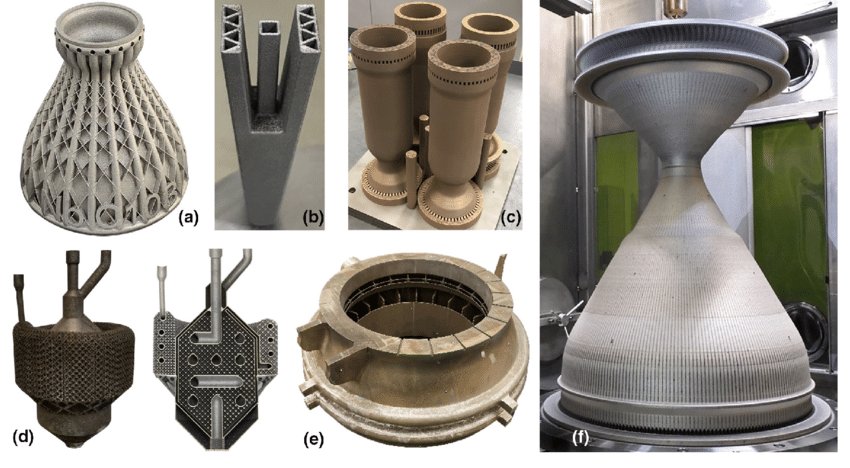
\includegraphics[width=.8\textwidth]{aero_2}
	\ccaption{Beispiele verschiedener Bauteile, welche mit \acrshort{am} produziert wurden}{\url{https://www.researchgate.net/profile/Paul-Gradl/publication/360032150/figure/fig4/AS:1146451094708236@1650346649497/Examples-of-complex-aerospace-parts-fabricated-with-different-metals-and-alloys-a.png}}
	\label{img:aero_1}
\end{figure} 

%\subsubsection{Automobil-Industrie}

\end{document}
